\documentclass[12pt]{article}
\renewcommand{\linespread}{1.5}
\usepackage[utf8x]{inputenc}
\usepackage[,english,greek]{babel}
\usepackage{amsmath}
\usepackage{listings}
\usepackage{tikz}
\usepackage{tikz-qtree}
\usetikzlibrary{arrows}
\begin{document}
	\begin{center}
    	\huge \textbf{Τεχνητή Νοημοσύνη \\ Εργασία 2}\\
    	\Large Κωνσταντίνος Χαϊδεμένος\\
    	\large $sdi2200262$\\ 
	\end{center}
\vspace{36pt}
\section*{Πρόβλημα 1}
Ισχυρισμός με λίγα λόγια:\\\\
Η χρησιμότητα του MAX εναντίον ενός μη βέλτιστου MIN δεν είναι ποτέ μικρότερη από την χρησιμότητα εναντίον ενός βέλτιστου MIN.\\\\
Ο ισχυρισμός φαίνεται αυτονόητος με την πρώτη ματιά.\\\\
Λαμβάνοντας υπόψην πως ο ΜΑΞ παίζει εναντίον ενός μη βέλτιστου ΜΙΝ ο οποίος κάνει λάθη, η στρατιγική του ΜΑΞ θα εκμεταλλευτεί αυτά τα λάθη και θα εγγυείται κάθε φορά την ίδια ή μεγαλύτερη χρησιμότητα από αυτήν που θα είχε ενάντια ενός βέλτιστου αντιπάλου.\\\\
Παρ΄όλα αυτά θα τον αποδείξουμε με απαγωγή σε άτοπο:\\\\
Ο στόχος του ΜΑΞ είναι να μεγιστοποιήσει την χρησιμότητά του και ο στόχος του ΜΙΝ είναι να ελαχιστοποιήσει την χρησιμότητα του ΜΑΞ.\\\\
Έστω πως παίζοντας ο ΜΑΞ ενάντια με έναν βέλτιστο αντίπαλο ΜΙΝ έχει χρησιμότητα $x$. Αυτό σημαίνει πως ο ΜΙΝ με την βέλτιστη στρατηγική του ελαχιστοποίησε την παραπάνω τιμή.\\\\
Έστω πως αμέσως μετά ο ΜΑΞ παίζει με έναν μη βέλτιστο αντίπαλο ΜΙΝ ωστόσο έχει χρησιμότητα $x' < x$. \\\\
Ώπα... άρα η στρατηγική του μη βέλτιστου ΜΙΝ ελαχιστοποίησε <<ακόμα περισσότερο>> την τιμή χρησιμότητας του ΜΑΞ?\\
Άρα είναι η πλέον βέλτιστη στρατηγική! Άρα Άτοποοοοο.\\\\
Ένα δένδρο παιχνιδιού στο οποίο ο ΜΑΞ έχει ακόμα καλύτερη χρησιμότητα, όμως με μη βέλτιστη στρατηγική και μη βέλτιστο αντίπαλο, είναι το εξής:\\\\
\begin{otherlanguage}{english}
\usetikzlibrary{trees}
\begin{tikzpicture}[
    edge from parent fork down,
    level 1/.style={sibling distance=3cm},
    level 2/.style={sibling distance=1.5cm},
    every node/.style={ draw, align=center, rounded corners}
  ]
    % Root
    \node[red] {\textbf{MAX}}
      % First child with 2 leaves
      child {node[red] {\textbf{MIN}}
        child {node {5}}
        child {node [red]{\textbf{20}}}
      }
      % Second child with 2 leaves
      child {node {MIN}
        child {node {10}}
        child {node {15}}
      };
\end{tikzpicture}
\end{otherlanguage}\\\\
Στο συγκεκριμένο δέντρο παιχνιδιού φαίνονται με \textbf{μπόλντ} \textcolor{red}{κόκκινα} γράμματα οι επιλογές των κινήσεων των MIN/MAX\\\\
Αυτή η ροή παιχνιδιού είναι αποτέλεσμα της στρατηγικής των ΜΑΞ και ΜΙΝ να διαλέγουν, από τους δύο κόμβους-επιλογές, πάντα αυτόν με την <<χειρότερη>> χρησιμότητα για τους ίδιους.\\\\
Επομένως αρχικά ο ΜΑΞ επιλέγει τον αριστερό ΜΙΝ κόμβο καθώς έχει το φύλλο του δέντρου με τη μικρότερη τιμή χρησιμότητας.\\\\
Τελικά όμως ο ΜΙΝ θα επιλέξει την τιμή 20 που προς έκπληξη όλων μας (εκτός από εμένα που σκέφτηκα αυτό το παράδειγμα ) είναι και το φύλλο του δέντρου με τη μεγαλύτερη τιμή χρησιμότητας!\\\\\\
\section*{Πρόβλημα 2}
α) \\
Το πλήρες δέντρο είναι ώς εξής:\\\\
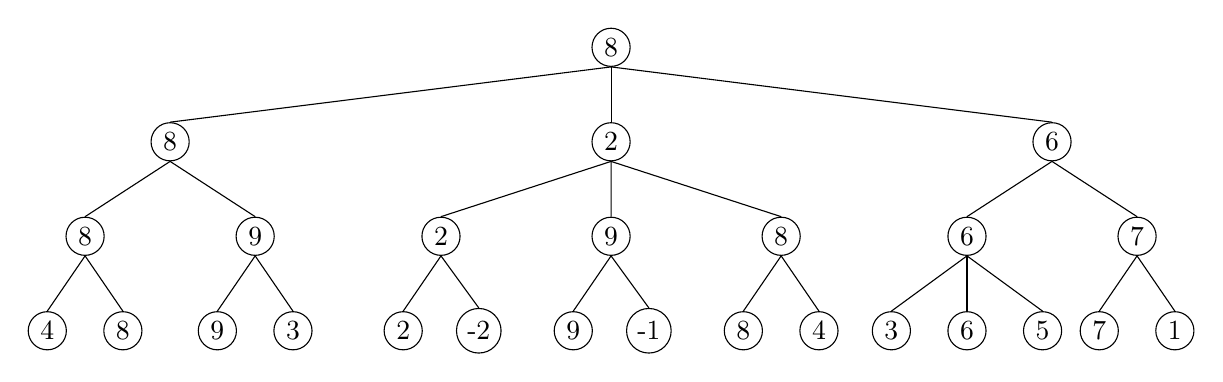
\begin{tikzpicture}[
scale=0.8, 
    level distance=1.5cm, 
    level 1/.style={sibling distance=7cm},
    level 2/.style={sibling distance=2.7cm},
    level 3/.style={sibling distance=1.2cm},
    every node/.style={circle,draw,inner sep=2pt,minimum size=1em},  size
    every leaf node/.style={circle,draw,inner sep=2pt,fill=gray!20,minimum size=1em}
]

\node {8}
    child {node {8}
        child {node {8}
            child {node {4}}
            child {node {8}}
        }
        child {node {9}
            child {node {9}}
            child {node {3}}
        }
    }
    child {node {2}
        child {node {2}
            child {node {2}}
            child {node {-2}}
        }
        child {node {9}
            child {node {9}}
            child {node {-1}}
        }
        child {node {8}
            child {node {8}}
            child {node {4}}
        }
    }
    child {node {6}
        child {node {6}
            child {node {3}}
            child {node {6}}
            child {node {5}}
        }
        child {node {7}
            child {node {7}}
            child {node {1}}
        }
    };

\end{tikzpicture}\\\\
β)
Η απόφαση $minimax$ στη ρίζα του δέντρου είναι να ακολουθήσει το μονοπάτι που καταλήγει στο κόμβο φύλλο με τιμή 8. Στο σχήμα φαίνεται με \textcolor{red}{κόκκινο}:\\\\
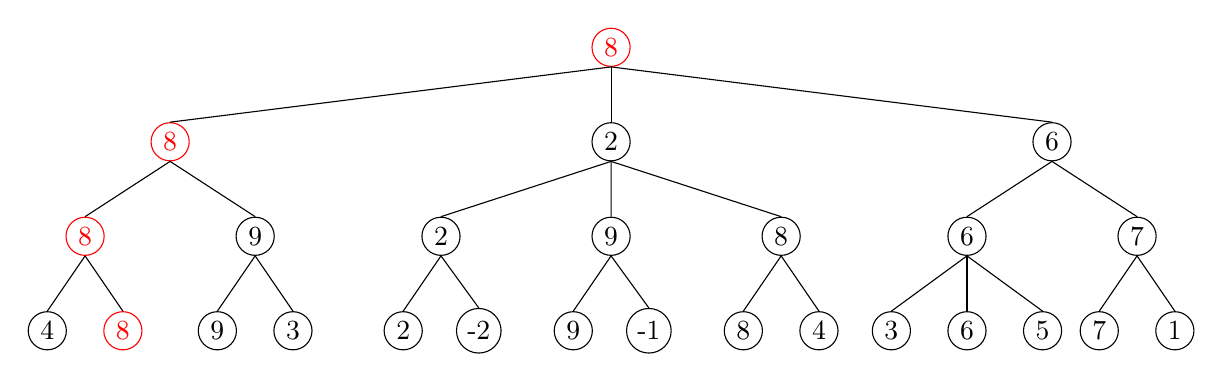
\begin{tikzpicture}[
scale=0.8, 
    level distance=1.5cm, 
    level 1/.style={sibling distance=7cm},
    level 2/.style={sibling distance=2.7cm},
    level 3/.style={sibling distance=1.2cm},
    every node/.style={circle,draw,inner sep=2pt,minimum size=1em},  size
    every leaf node/.style={circle,draw,inner sep=2pt,fill=gray!20,minimum size=1em}
]

\node [red] {8}
    child {node[red] {8}
        child {node [red]{8}
            child {node {4}}
            child {node [red]{8}}
        }
        child {node {9}
            child {node {9}}
            child {node {3}}
        }
    }
    child {node {2}
        child {node {2}
            child {node {2}}
            child {node {-2}}
        }
        child {node {9}
            child {node {9}}
            child {node {-1}}
        }
        child {node {8}
            child {node {8}}
            child {node {4}}
        }
    }
    child {node {6}
        child {node {6}
            child {node {3}}
            child {node {6}}
            child {node {5}}
        }
        child {node {7}
            child {node {7}}
            child {node {1}}
        }
    };

\end{tikzpicture}\\\\
γ)
Εφαρμόζοντας τον αλγόριθμο $alpha$ $beta$ $search$ στο δέντρο του προβλήματος ξεκινόντας από τα αριστερά θα έχουμε με \textcolor{blue}{μπλέ} τους κόμβους που κόπηκαν:\\\\

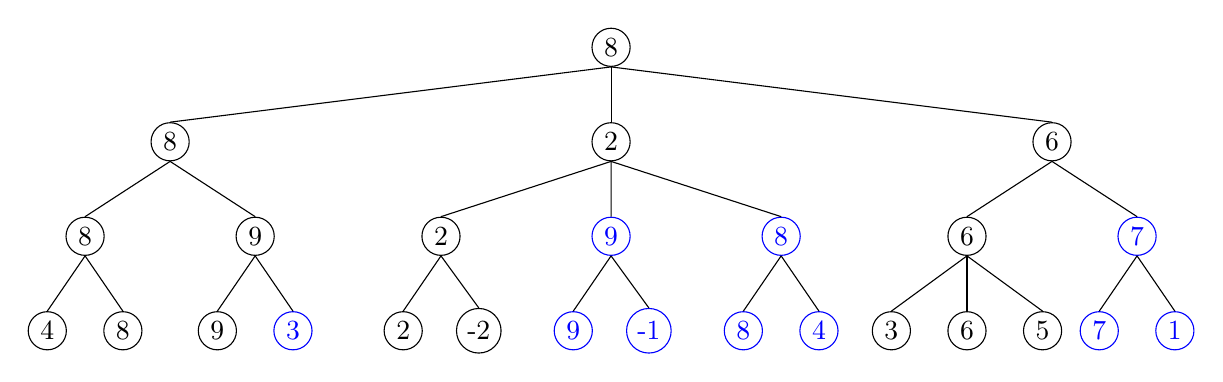
\begin{tikzpicture}[
scale=0.8, 
    level distance=1.5cm, 
    level 1/.style={sibling distance=7cm},
    level 2/.style={sibling distance=2.7cm},
    level 3/.style={sibling distance=1.2cm},
    every node/.style={circle,draw,inner sep=2pt,minimum size=1em},  size
    every leaf node/.style={circle,draw,inner sep=2pt,fill=gray!20,minimum size=1em}
]

\node {8}
    child {node {8}
        child {node {8}
            child {node {4}}
            child {node {8}}
        }
        child {node {9}
            child {node {9}}
            child {node [blue]{3}}
        }
    }
    child {node {2}
        child {node {2}
            child {node {2}}
            child {node {-2}}
        }
        child {node[blue] {9}
            child {node [blue]{9}}
            child {node [blue]{-1}}
        }
        child {node[blue] {8}
            child {node [blue]{8}}
            child {node [blue]{4}}
        }
    }
    child {node {6}
        child {node {6}
            child {node {3}}
            child {node {6}}
            child {node {5}}
        }
        child {node[blue] {7}
            child {node [blue]{7}}
            child {node [blue]{1}}
        }
    };

\end{tikzpicture}
\section*{Πρόβλημα 3}
α)\\
Το δέντρο φαίνεται στο παρακάτω σχήμα. O έντονα χρωματισμένος κόμβος τύχης αποτελεί την καλύτερη κίνηση για την ρίζα:\\\\
\begin{center}
    
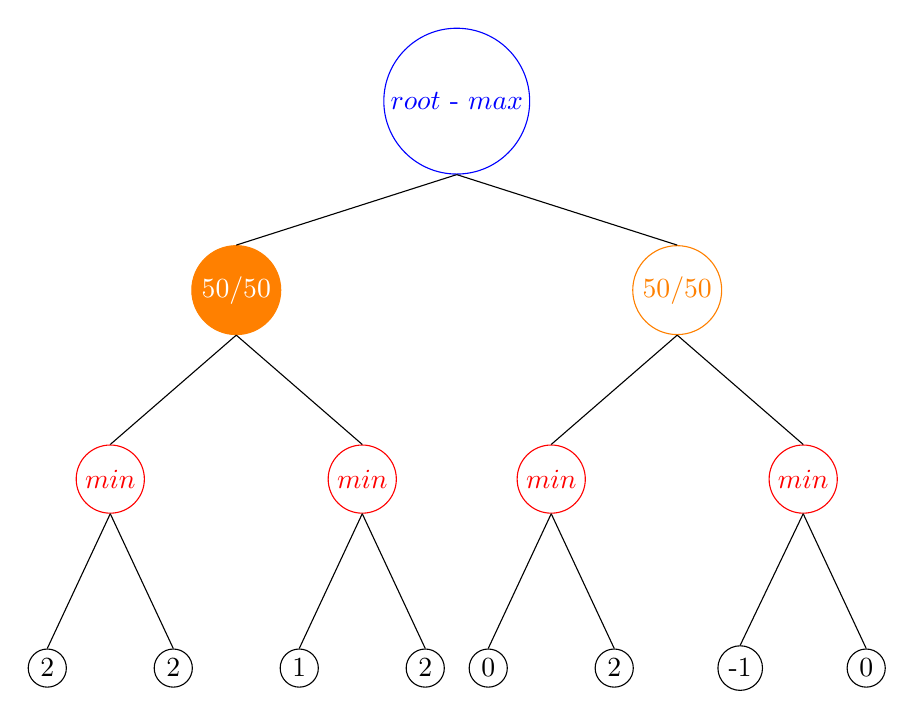
\begin{tikzpicture}[
scale=0.8, 
    level distance=3cm, 
    level 1/.style={sibling distance=7cm},
    level 2/.style={sibling distance=4cm},
    level 3/.style={sibling distance=2cm},
    every node/.style={circle,draw,inner sep=2pt,minimum size=1em},  size
    every leaf node/.style={circle,draw,inner sep=2pt,fill=gray!20,minimum size=1em}
]

\node [blue]{$root$ - $max$}
        child {node [fill] [orange]{\textcolor{white}{50/50}}
            child {node [red]{$min$}
                child{node {2}}
                child{node {2}}
            }
            child {node [red]{$min$}
                child{node{1}}
                child{node{2}}
            }
        }
        child {node [orange] {50/50}
            child {node [red]{$min$}
                child{node{0}}
                child{node{2}}
            }
            child {node [red]{$min$}
                child{node{-1}}
                child{node{0}}
            }
        };
\end{tikzpicture}
\end{center}
Για να αποφασίσουμε ποιόν κόμβο τύχης θα επιλέξει η ρίζα πρέπει να βρούμε την αναμενόμενη $evaluation$ τιμή για κάθε $branch$.\\\\
Απλά παίρνουμε το άθροισμα των τιμών των κόμβων-φύλλα για το κάθε $branch$ και το διαιρούμε με 2. Ο μεγαλύτερος αριθμός από τους δύο που θα προκύψουν θα μας οδηγήσει στην πιο κατάλληλη κίνηση για την ρίζα.\\\\
Με άλλα λόγια η ρίζα έχει μεγαλύτερη <<πιθανότητα>> να πετύχει υψηλότερη  $evaluation$ τιμή αν επιλέξει τον αριστερό κόμβο τύχης, καθώς οι τιμές στα φύλλα από εκείνο το $branch$ είναι κατά μέσο όρο υψηλότερες.\\\\\\\\\\
β)\\
\underline{Περίπτωση 1:} Γνωρίζουμε τις τιμές των πρώτων 6 κόμβων\\\\
Στη συγκεκριμένη περίπτωση δεν μπορούμε να καταλήξουμε σε ποιό κόμβο-φύλλο θα επιλέξει ο 4ος κόμβος $min$ επομένως δεν ξέρουμε την τιμή του δεξιού κόμβου-τύχης.\\\\
Άρα δεν θα μπορούμε να βρούμε με σιγουριά την κατάλληλη επιλογή της ρίζας.\\\\\\
\underline{Περίπτωση 2:} Γνωρίζουμε τις τιμές των πρώτων 7 κόμβων\\\\
Εδώ διακρίνουμε δύο υποπεριπτώσεις:
\begin{itemize}
    \item τιμή 8ου κόμβου $\geq$ 0\\\\
    Τότε προφανώς ο 4ος $min$ επιλέγει την τιμή -1 και έπειτα η τιμή του δεξιού κόμβου-τύχης υπολογίζεται σε -0.5. Άααααρα ο η καλύτερη επιλογή της ρίζας είναι να πάει αριστερά πάλι.\\
    \item τιμή 8ου κόμβου $<$ 0 \\\\
    Τότε δεν ξέρουμε ποιόν θα διαλέξει ο 4ος $min$, ωστόσο είναι προφανές πως η τιμή του δεξιού κόμβου-τύχης θα είναι ξανά αρνητική. Επομένως πάλι η καλύτερη επιλογή της ρίζας είναι να πάει αριστερά.\\\\   
\end{itemize}
γ)\\
Τα δύο πρώτα φύλλα του δέντρου έχουν τιμές 2 και 2. Επομένως, υποθέτοντας πως ο $min$ κόμβος σε περίπτωση ισοτιμίας διαλέγει τον αριστερότερο κόμβο, η τιμή του πρώτου $min$ είναι 2.\\\\
Οι δυνατές τιμές του αριστερού κόμβου-τύχης εξαρτούνται από το σύνολο τιμών του δεύτερου $min$ κόμβου. Από την εκφώνηση γνωρίζουμε πως το σύνολο αυτό είναι $[-2,2]$.\\\\
Διακρίνουμε λοιπόν, πάλι δύο ακραίες περιπτώσεις:\\
\begin{itemize}
    \item Το 3ο και το 4ο φύλλο έχουν τιμές -2 και η τελική τιμή του 2ου $min$ κόμβου είναι -2:\\
    Σε αυτή τη περίπτωση η τιμή του αριστερού κόμβου τύχης είναι 0.
    \item Το 3ο και το 4ο φύλλο έχουν τιμές 2 και η τελική τιμή του 2ου $min$ κόμβου είναι 2:\\
    Σε αυτή τη περίπτωση η τιμή του αριστερού κόμβου τύχης είναι 2.
\end{itemize}
Εφόσον ο 2ος κόμβος $min$ μπορεί να πάρει οποιαδήποτε τιμή μεταξύ -2 και 2 και οι ακραίες τιμές του αριστερού κόμβου τύχης είναι 0 και 2, συμπεραίνουμε πως οι δυνατές τιμές του αριστερού κόμβου τύχης είναι το σύνολο [0,2].\\\\\\\\
δ)\\
Στο παρακάτω δέντρο συμβολίζονται με Χ οι κόμβοι τους οποίους δεν θα επισκεφτεί ο αλγόριθμος κλάδεμα - ΑΒ:\\
\begin{center}
    
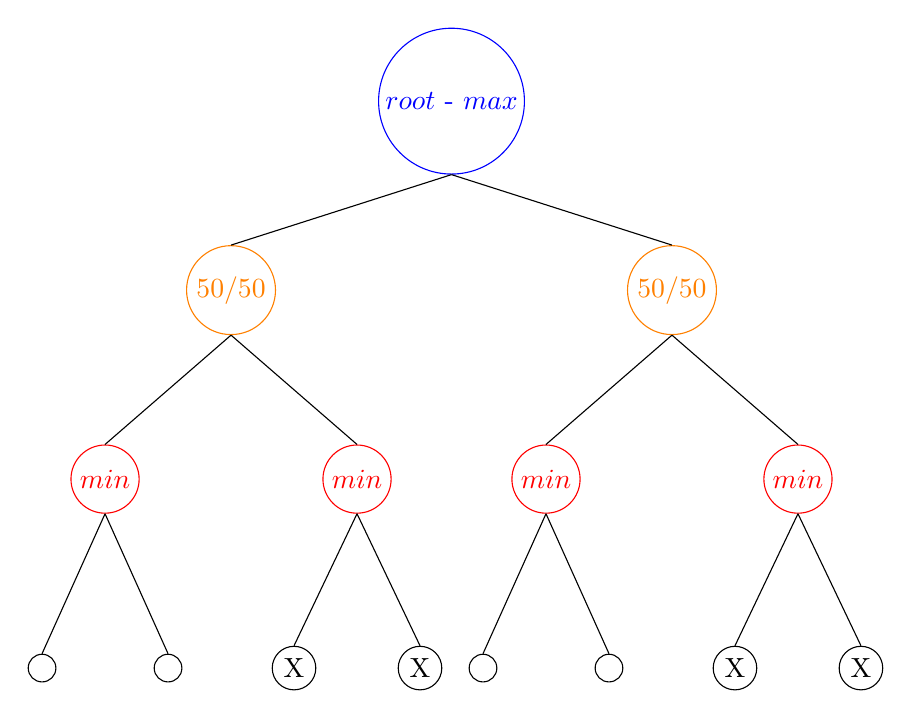
\begin{tikzpicture}[
scale=0.8, 
    level distance=3cm, 
    level 1/.style={sibling distance=7cm},
    level 2/.style={sibling distance=4cm},
    level 3/.style={sibling distance=2cm},
    every node/.style={circle,draw,inner sep=2pt,minimum size=1em},  size
    every leaf node/.style={circle,draw,inner sep=2pt,fill=gray!20,minimum size=1em}
]

\node [blue]{$root$ - $max$}
        child {node  [orange]{50/50}
            child {node [red]{$min$}
                child{node {}}
                child{node {}}
            }
            child {node [red]{$min$}
                child{node{Χ}}
                child{node{Χ}}
            }
        }
        child {node [orange] {50/50}
            child {node [red]{$min$}
                child{node{}}
                child{node{}}
            }
            child {node [red]{$min$}
                child{node{Χ}}
                child{node{Χ}}
            }
        };
\end{tikzpicture}
\end{center}
Όπως διαπιστώσαμε στο ερώτημα (γ) άν γνωρίζουμε το σύνολο τιμών τών φύλλων, γνωρίζουμε αυτόματα το σύνολο τιμών του κάθε $min$ κόμβου και τις δυνατές τιμές του κάθε κόμβου-τύχης.\\\\
Στη συγκεκριμένη περίπτωση διαπιστώνουμε, εφαρμόζοντας την ίδια λογική με το προηγούμενο ερώτημα, πως οι δυνατές τιμές του αριστερού-κόμβου τύχης είναι [-2,2]. Το ίδιο συμβαίνει και με τον δεξιά κόμβο-τύχης.\\\\
Στην περίπτωση που γίνεται κλάδεμα - ΑΒ αρκεί για κάθε κόμβο τύχης να ελεγχτούν μόνο οι τιμές των φύλλων του αριστερού παιδιού $min$.\\\\
\section*{Πρόβλημα 4}
α)\\
Το δέντρο του παιχνιδιού $Νim$ με τον πρώτο παίκτη να είναι ο $MAX$ είναι:\\\\
με \textcolor{red}{κοκκινο} οι μαξ κόμβοι\\
και με \textcolor{blue}{μπλε} οι μιν κόμβοι\\\\
\begin{center}
    
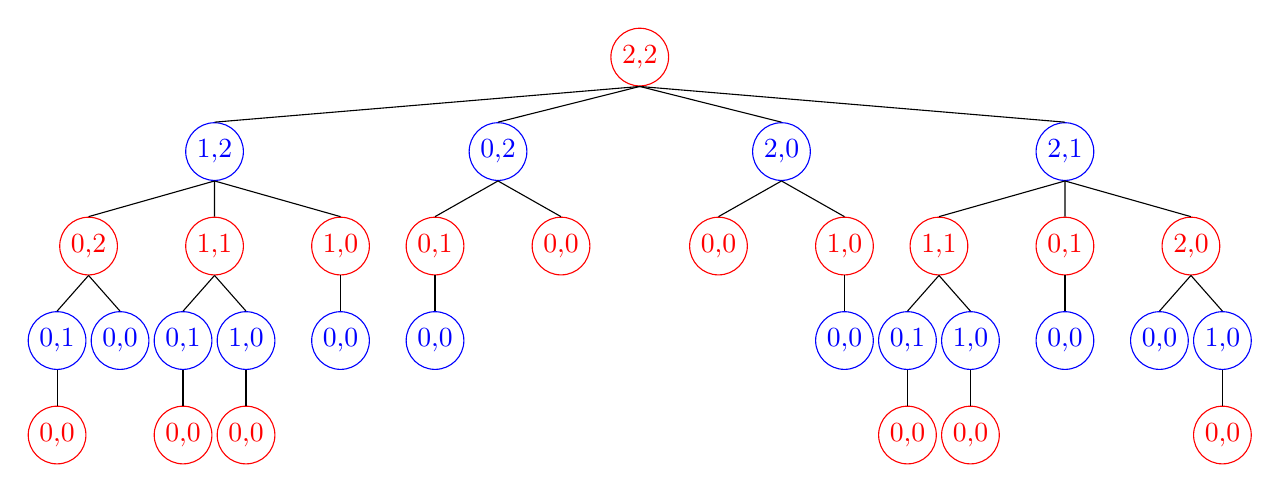
\begin{tikzpicture}[
scale=0.8, 
    level distance=1.5cm, 
    level 1/.style={sibling distance=4.5cm},
    level 2/.style={sibling distance=2cm},
    level 3/.style={sibling distance=1cm},
    every node/.style={circle,draw,inner sep=2pt,minimum size=1em},  size
    every leaf node/.style={circle,draw,inner sep=2pt,fill=gray!20,minimum size=1em}
]

\node [red] {2,2}
    child {node [blue] {1,2}
        child {node [red] {0,2}
            child {node [blue] {0,1}
                child{node [red] {0,0}}
                }
            child {node [blue] {0,0}}
        }
        child {node [red] {1,1}
            child {node [blue] {0,1}
                child{node [red] {0,0}}
                }
            child {node [blue] {1,0}
                child{node [red] {0,0}}
                }
        }
        child {node [red] {1,0}
            child {node [blue] {0,0}}
        }
    }
    child {node [blue] {0,2}
        child {node [red] {0,1}
            child {node [blue] {0,0}}
        }
        child {node [red] {0,0}}
    }
    child {node [blue] {2,0}
        child {node [red] {0,0}}
        child {node [red] {1,0}
            child {node [blue] {0,0}}
        }
    }
    child {node [blue] {2,1}
        child {node [red] {1,1}
            child {node [blue] {0,1}
                child{node[red] {0,0}}
                }
            child {node [blue] {1,0}
                child{node [red] {0,0}}
                }
        }
        child {node [red] {0,1}
            child {node [blue] {0,0}}
        }
        child {node [red] {2,0}
            child {node [blue] {0,0}}
            child {node [blue] {1,0}
                child{node [red] {0,0}}
                }
        }
    };

\end{tikzpicture}
\end{center}
\end{document}